\subsection{Sequences, Countability, and Metrization}

Countability axioms control when topological questions can be reduced to sequences and countable tests. They also separate metric phenomena from genuinely non-metric topologies.

\begin{definition} \label{def:topological-sequence-convergence} \hlt{Sequence Convergence and Sequential Compactness}\\
A sequence $(x_n)$ in a topological space $X$ \hlt{converges} to $x\in X$ if for every neighborhood $U$ of $x$ there is $N$ such that $x_n\in U$ whenever $n\geq N$.\\
The space $X$ is \hlt{sequentially compact} if every sequence in $X$ has a subsequence that converges to a point of $X$.
\end{definition}

\begin{proposition} \label{prop:hausdorff-sequence-limits-unique} \hlt{Hausdorff Sequence Limits Are Unique}\\
In a Hausdorff space, a sequence has at most one limit. In the trivial topology, every sequence converges to every point.
\begin{proof}
If $x_n\to x$ and $x_n\to y$ with $x\neq y$ in a Hausdorff space, choose disjoint neighborhoods $U$ of $x$ and $V$ of $y$. Eventually $x_n\in U$ and eventually $x_n\in V$, impossible because $U\cap V=\emptyset$. In the trivial topology, the only neighborhood of any point is $X$, so every sequence is eventually in every neighborhood.\\
\hlt{Key Insight}: Hausdorff separation prevents one tail of a sequence from living near two distinct points.
\end{proof}
\end{proposition}

\begin{definition} \label{def:topological-countability-axioms} \hlt{Countability Axioms}\\
A topological space $(X,\tau)$ is:
\begin{enumerate}[label=(\roman*)]
\setlength{\itemsep}{0pt}
\item \hlt{first countable} if each $x\in X$ admits a countable neighborhood basis $\mathcal{B}_x$.\\
For every neighborhood $U\ni x$, $\exists B\in\mathcal{B}_x$ with $B\subseteq U$;
\item \hlt{second countable} if $\tau$ has a countable basis;
\item \hlt{separable} if there is a countable dense subset $D\subseteq X$, equivalently $\overline{D}=X$ or every nonempty open set meets $D$.
\end{enumerate}
\end{definition}

\begin{example} \label{ex:metric-spaces-first-countable} \hlt{Metric Spaces Are First Countable}\\
Every metric space is first countable: for each $x$, the balls $\{B_{1/n}(x):n\geq1\}$ form a countable neighborhood basis at $x$.
\end{example}

\begin{proposition} \label{prop:second-countable-implies-first-countable} \hlt{Second Countable Implies First Countable}\\
Every second countable space is first countable.
\begin{proof}
Let $\mathcal{B}$ be a countable basis for the topology. For $x\in X$, the subcollection $\mathcal{B}_x\defeq\{B\in\mathcal{B}:x\in B\}$ is countable. If $U$ is a neighborhood of $x$, choose $B\in\mathcal{B}$ with $x\in B\subseteq U$. Hence $\mathcal{B}_x$ is a countable neighborhood basis at $x$.\\
\hlt{Key Insight}: A global countable basis restricts to countable local bases.
\end{proof}
\end{proposition}

\begin{proposition} \label{prop:second-countable-implies-separable} \hlt{Second Countable Consequences}\\
If $(X,\tau)$ is second countable, then there is a countable $D\subseteq X$ with $\overline{D}=X$. Moreover, every subspace of a second countable space is second countable.
\begin{proof}
Let $\mathcal{B}=\{B_n:n\in I\}$ be a countable basis, with $I\subseteq\N$.\\
For each $n\in I$ with $B_n\neq\emptyset$, choose $x_n\in B_n$ and set $D=\{x_n:n\in I,\ B_n\neq\emptyset\}$. Then $D$ is countable.\\
If $U\in\tau\setminus\{\emptyset\}$, choose $x\in U$; some $B_n\in\mathcal{B}$ satisfies $x\in B_n\subseteq U$, so $x_n\in D\cap U$. Hence $\overline{D}=X$.\\
If $Y\subseteq X$, then $\{B_n\cap Y:n\in I\}$ is a countable basis for the subspace topology on $Y$.\\
\hlt{Structural Commentary}: $\mathcal{B}$ countable gives countable $D$ meeting every $U\in\tau\setminus\{\emptyset\}$.\\
\hlt{Key Insight}: $D$ is dense iff $D\cap U\neq\emptyset$ for every $U\in\tau\setminus\{\emptyset\}$.
\end{proof}
\end{proposition}

\begin{proposition} \label{prop:first-countable-sequential-closure} \hlt{First Countable Sequential Closure}\\
Let $X$ be first countable, $E\subseteq X$, and $x\in X$. Then $x\in\overline{E}$ iff $x$ is the limit of a sequence in $E$. Consequently, $E$ is closed iff every convergent sequence in $E$ has all its limits in $E$.
\begin{proof}
If $x_n\in E$ and $x_n\to x$, then every neighborhood of $x$ contains a tail of the sequence and therefore meets $E$, so $x\in\overline{E}$. Conversely, let $\{B_n:n\geq1\}$ be a countable neighborhood basis at $x$. Since $x\in\overline{E}$ and $\bigcap_{j=1}^nB_j$ is a neighborhood of $x$, choose
\[
x_n\in E\cap\bigcap_{j=1}^nB_j.
\]
Then $x_n\to x$. The closed-set criterion follows from Proposition \ref{prop:topological-closure-closed-calculus}.\\
\hlt{Key Insight}: First countability turns all neighborhood tests into one sequence of tests.
\end{proof}
\end{proposition}

\begin{example} \label{ex:uncountable-cofinite-topology-not-first-countable} \hlt{Uncountable Cofinite Topology}\\
Let $X$ be uncountable and let $\tau$ consist of $\emptyset$ together with all subsets of $X$ whose complements are finite. Then $\tau$ is a topology, it is $T_1$, and it is not first countable.
\begin{proof}
Finite intersections and arbitrary unions of cofinite sets are cofinite, so $\tau$ is a topology. Since $X\setminus\{x\}$ is open for each $x$, singletons are closed, so Proposition \ref{prop:t1-iff-singletons-closed} applies.\\
Fix $x\in X$. If $\{B_n:n\geq1\}$ were a countable neighborhood basis at $x$, then each $X\setminus B_n$ would be finite. The union $\bigcup_n(X\setminus B_n)$ is countable, so choose $y\in X\setminus\left(\{x\}\cup\bigcup_n(X\setminus B_n)\right)$. Then $U=X\setminus\{y\}$ is a neighborhood of $x$, but no $B_n$ is contained in $U$ because $y\in B_n$ for every $n$.\\
\hlt{Key Insight}: Cofinite neighborhoods are too large to be compressed into countably many local tests at a point.
\end{proof}
\end{example}

\begin{definition} \label{def:lindelof-space} \hlt{Lindel\"of Space}\\
A topological space $X$ is \hlt{Lindel\"of} if every open cover of $X$ has a countable subcover.
\end{definition}

\begin{definition} \label{def:countably-compact-space} \hlt{Countably Compact Space}\\
A topological space $X$ is \hlt{countably compact} if every countable open cover of $X$ has a finite subcover.
\end{definition}

\begin{proposition} \label{prop:countably-compact-frechet-intersection} \hlt{Frechet Intersection Test for Countable Compactness}\\
A topological space $X$ is countably compact iff every descending sequence
\[
F_1\supseteq F_2\supseteq\cdots
\]
of nonempty closed subsets of $X$ has nonempty intersection.
\begin{proof}
Assume $X$ is countably compact. If $\bigcap_nF_n=\emptyset$, then $\{X\setminus F_n:n\geq1\}$ is a countable open cover of $X$. A finite subcover exists, and since the $F_n$ are descending, one member $X\setminus F_N$ already covers $X$, contradicting $F_N\neq\emptyset$.\\
Conversely, let $\{O_n:n\geq1\}$ be a countable open cover with no finite subcover. Put
\[
F_n\defeq X\setminus(O_1\cup\cdots\cup O_n).
\]
Then the $F_n$ are nonempty, closed, and descending, but their intersection is empty.\\
\hlt{Key Insight}: Countable compactness is the open-cover form of the nested closed-set principle.
\end{proof}
\end{proposition}

\begin{theorem} \label{thm:dini-countably-compact} \hlt{Dini's Theorem on Countably Compact Spaces}\\
Let $X$ be countably compact, and let $f_n:X\to\R$ be continuous with $f_n(x)\downarrow0$ for every $x\in X$. Then $f_n\to0$ uniformly on $X$.
\begin{proof}
Fix $\varepsilon>0$ and set $O_n\defeq\{x\in X:f_n(x)<\varepsilon\}$. Each $O_n$ is open, and monotonicity gives $O_n\subseteq O_{n+1}$. Since $f_n(x)\downarrow0$ pointwise, the $O_n$ cover $X$ and $f_n(x)\geq0$ for all $n,x$. Countable compactness gives a finite subcover; because the cover is increasing, some $O_N$ already equals $X$. Hence $0\leq f_n(x)\leq f_N(x)<\varepsilon$ for all $x\in X$ and all $n\geq N$.\\
\hlt{Key Insight}: A monotone pointwise estimate turns the countable open cover $\{f_n<\varepsilon\}$ into one global index.
\end{proof}
\end{theorem}

\begin{proposition} \label{prop:second-countable-implies-lindelof} \hlt{Second Countable Implies Lindel\"of}\\
Every second countable space is Lindel\"of.
\begin{proof}
Let $\mathcal{B}=\{B_n:n\in I\}$ be a countable basis and let $\mathcal{U}$ be an open cover of $X$. For each $B_n$ that is contained in at least one member of $\mathcal{U}$, choose one such $U_n\in\mathcal{U}$. The selected family is countable. If $x\in X$, choose $U\in\mathcal{U}$ with $x\in U$, then choose $B_n$ with $x\in B_n\subseteq U$. Thus $U_n$ is selected and contains $x$.\\
\hlt{Key Insight}: A countable basis reduces an arbitrary open cover to countably many basis elements.
\end{proof}
\end{proposition}

\begin{proposition} \label{prop:second-countable-countably-compact-compact} \hlt{Second Countable Countable Compactness Is Compactness}\\
For a second countable topological space, compactness is equivalent to countable compactness.
\begin{proof}
Compactness immediately implies countable compactness. Conversely, if $X$ is second countable, Proposition \ref{prop:second-countable-implies-lindelof} gives a countable subcover for every open cover; countable compactness then extracts a finite subcover.\\
\hlt{Key Insight}: Second countability lowers arbitrary covers to countable covers.
\end{proof}
\end{proposition}

\begin{theorem} \label{thm:second-countable-compact-iff-sequentially-compact} \hlt{Second Countable Compactness and Sequential Compactness}\\
Let $X$ be second countable. Then $X$ is compact iff $X$ is sequentially compact.
\begin{proof}
Assume $X$ is compact and let $(x_n)$ be a sequence. For $n\geq1$, set $F_n=\overline{\{x_k:k\geq n\}}$. The sets $F_n$ are closed, nonempty, and descending, so Proposition \ref{prop:topological-compactness-fip} gives $x\in\bigcap_nF_n$. By Proposition \ref{prop:second-countable-implies-first-countable}, choose a descending countable neighborhood basis $(B_j)$ at $x$. Set $n_0=0$; after $n_{j-1}$ has been chosen, use $x\in F_{n_{j-1}+1}$ and the neighborhood $B_j$ to choose $n_j>n_{j-1}$ with $x_{n_j}\in B_j$. Then $x_{n_j}\to x$.\\
Conversely, assume $X$ is sequentially compact. By Proposition \ref{prop:second-countable-implies-lindelof}, it suffices to show every countable open cover $\{O_n\}_{n\geq1}$ has a finite subcover. If none does, choose $x_n\notin O_1\cup\cdots\cup O_n$. A subsequence $x_{n_j}$ converges to some $x\in X$, and $x\in O_N$ for some $N$. Since $O_N$ is a neighborhood of $x$, eventually $x_{n_j}\in O_N$, contradicting $x_n\notin O_N$ for all $n\geq N$.\\
\hlt{Key Insight}: Second countability supplies enough sequences to recover compactness.
\end{proof}
\end{theorem}

\begin{example} \label{ex:sorgenfrey-line-countability-tests} \hlt{The Sorgenfrey Line}\\
Let $\mathcal{B}=\{[a,b):a<b\}$ on $\R$. Then $\mathcal{B}$ is a basis for a topology, called the \hlt{Sorgenfrey line}. This space is first countable and separable, but it is not second countable and therefore is not metrizable.
\begin{proof}
The intervals $[a,b)$ cover $\R$. If $x\in[a,b)\cap[c,d)$, then $x\in[x,e)\subseteq[a,b)\cap[c,d)$ for some $e>x$, so $\mathcal{B}$ is a basis. The countable family $\{[x,x+1/n):n\geq1\}$ is a neighborhood basis at $x$, hence the space is first countable. Every nonempty basis interval $[a,b)$ contains a rational number, so $\Q$ is dense.\\
If $\mathcal{C}$ were a countable basis for the Sorgenfrey topology, then for each $x\in\R$ choose $C_x\in\mathcal{C}$ such that
\[
x\in C_x\subseteq[x,x+1).
\]
If $x<y$, then $C_y\subseteq[y,y+1)$ cannot contain $x$, whereas $x\in C_x$, so $C_x\neq C_y$. This gives an uncountable subfamily of $\mathcal{C}$, impossible. Thus the space is not second countable. If it were metrizable, separability and Proposition \ref{prop:metric-separable-countable-base} would imply second countability, a contradiction.\\
\hlt{Key Insight}: First countability is local, while second countability requires one countable basis to remember all left endpoints.
\end{proof}
\end{example}

\begin{example} \label{ex:moore-plane-countability-and-metrizability} \hlt{The Moore Plane}\\
Let
\[
\mathbb{M}\defeq\{(x,y)\in\R^2:y\geq0\}.
\]
For $y>0$, use ordinary Euclidean open balls contained in $\mathbb{M}$ as basic neighborhoods of $(x,y)$. For a boundary point $(x,0)$, use sets consisting of $(x,0)$ together with the points of a Euclidean open disk in the upper half-plane tangent to the boundary line at $(x,0)$. These basic neighborhoods define the \hlt{Moore plane}.
\begin{proof}
The basis axioms follow by shrinking Euclidean disks. At boundary points, two tangent disks based at the same point contain a smaller tangent disk, and an interior point lying in a tangent disk has a small Euclidean ball contained in the same tangent disk.\\
The space is Hausdorff: distinct interior points are separated by small Euclidean balls; distinct boundary points are separated by sufficiently small tangent disks; and an interior point and a boundary point are separated by shrinking the Euclidean ball and the tangent disk.\\
The Moore plane is separable, since rational points with positive rational height meet every basic neighborhood. However the boundary line $\R\times\{0\}$ is an uncountable discrete subspace: the intersection of a boundary tangent neighborhood with $\R\times\{0\}$ is the singleton base point. Thus the boundary subspace is not separable. If $\mathbb{M}$ were second countable, this subspace would be second countable and hence separable by Proposition \ref{prop:second-countable-implies-separable}, a contradiction. Since $\mathbb{M}$ is separable, metrizability would also force second countability by Proposition \ref{prop:metric-separable-countable-base}; hence the Moore plane is not metrizable.\\
\hlt{Key Insight}: The upper half-plane has many rational points, but the tangent boundary neighborhoods make the entire boundary line discrete as a subspace.
\end{proof}
\end{example}

\begin{figure}[H]
  \centering
  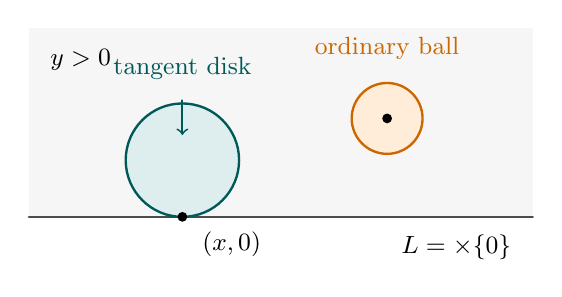
\begin{tikzpicture}[
  scale=1.0,
  every node/.style={font=\small},
  line cap=round,
  line join=round,
  upper/.style={fill=gray!7},
  boundary/.style={line width=0.85pt, black!70},
  tangent/.style={draw=teal!70!black, fill=teal!13, line width=0.85pt},
  ordinary/.style={draw=orange!80!black, fill=orange!15, line width=0.85pt},
  guide/.style={->, teal!70!black, line width=0.65pt},
  point/.style={circle, fill=black, inner sep=1.25pt}
]
\fill[upper] (-3.2,0) rectangle (3.2,2.4);
\draw[boundary] (-3.2,0) -- (3.2,0);
\node[anchor=north west] at (-3.05,2.25) {$y>0$};
\node[anchor=north east] at (3.05,-0.10) {$L=\R\times\{0\}$};

\draw[tangent] (-1.25,0.72) circle (0.72);
\node[teal!70!black, anchor=south] at (-1.25,1.62) {tangent disk};
\draw[guide] (-1.25,1.48) -- (-1.25,1.04);
\node[point] at (-1.25,0) {};
\node[anchor=north west] at (-1.12,-0.06) {$(x,0)$};

\draw[ordinary] (1.35,1.25) circle (0.45);
\node[orange!80!black, anchor=south] at (1.35,1.88) {ordinary ball};
\node[point] at (1.35,1.25) {};
\end{tikzpicture}

  \caption{A Moore-plane boundary neighborhood is a tangent disk together with its tangent boundary point.}
  \label{fig:moore-plane-basic-neighborhoods}
\end{figure}

\begin{definition} \label{def:metrizable-topological-space} \hlt{Metrizable Space}\\
A topological space is \hlt{metrizable} if its topology is induced by some metric.
\end{definition}

\begin{theorem} \label{thm:urysohn-metrization-second-countable} \hlt{Urysohn Metrization Theorem}\\
Let $X$ be second countable. Then $X$ is metrizable iff it is normal in the sense of Definition \ref{def:separation-axioms}.
\begin{proof}
If the topology is induced by a metric, Proposition \ref{prop:metric-spaces-are-normal} gives normality. Conversely, assume $X$ is second countable and normal, and let $\{U_n:n\in\N\}$ be a countable basis. Put
\[
A\defeq\{(n,m)\in\N\times\N:\overline{U_n}\subseteq U_m\}.
\]
For each $(n,m)\in A$, Urysohn's lemma, Theorem \ref{thm:urysohn-lemma-normal-space}, gives a continuous $f_{n,m}:X\to[0,1]$ with $f_{n,m}=0$ on $\overline{U_n}$ and $f_{n,m}=1$ on $X\setminus U_m$. Define
\[
\rho(x,y)\defeq\sum_{(n,m)\in A}\frac{1}{2^{n+m}}\abs{f_{n,m}(x)-f_{n,m}(y)}.
\]
This sum converges and defines a pseudometric. It separates distinct points: if $x\neq y$, normality first gives an open neighborhood $G$ of $x$ with $y\notin G$. Choose a basis element $U_m$ with $x\in U_m\subseteq G$, then use Proposition \ref{prop:normality-nested-neighborhoods} and the basis to choose $U_n$ with
\[
x\in U_n\subseteq\overline{U_n}\subseteq U_m.
\]
Then $(n,m)\in A$, while $y\notin U_m$, so $f_{n,m}(x)=0$, $f_{n,m}(y)=1$, and $\rho(x,y)>0$. Thus $\rho$ is a metric.\\
For fixed $x$, the defining series for $y\mapsto\rho(x,y)$ converges uniformly by comparison with $\sum_{n,m}2^{-(n+m)}$, so every $\rho$-ball is open in the original topology. Conversely, let $G$ be an original open neighborhood of $x$. Choose $U_m$ with $x\in U_m\subseteq G$, and choose $U_n$ with $x\in U_n\subseteq\overline{U_n}\subseteq U_m$. If $y\notin U_m$, then $f_{n,m}(x)=0$ and $f_{n,m}(y)=1$, so $\rho(x,y)\geq2^{-(n+m)}$. Hence the $\rho$-ball of radius $2^{-(n+m+1)}$ around $x$ lies in $U_m\subseteq G$. The metric topology is therefore the original topology.\\
\hlt{Key Insight}: Urysohn functions supply countably many coordinate tests that separate points and recover the topology.
\end{proof}
\end{theorem}
